%!Tex Program = xelatex
%------------------------------------------------------------------------------%
% Compile this document, by following instructures below:
% > xelatex assignment.tex
% > xelatex assignment.tex
% > bibtex assignment.aux
% > xelatex assignment.tex
%------------------------------------------------------------------------------%
\documentclass{article}
% pdf 设置区
%---------------------------------纸张大小设置---------------------------------%
\usepackage{geometry}
\geometry{a4paper,left=1.91cm,right=1.91cm,top=2.05cm,bottom=2.05cm}
%------------------------------------------------------------------------------%


%----------------------------------必要库支持----------------------------------%
\usepackage{xcolor}
\usepackage{tikz}
\usepackage{layouts}
\usepackage[numbers,sort&compress]{natbib}
\usepackage{clrscode}
\usepackage{gensymb}
%------------------------------------------------------------------------------%


%--------------------------------添加书签超链接--------------------------------%
\usepackage[unicode=true,colorlinks=false,pdfborder={0 0 0}]{hyperref}
% 在此处修改打开文件操作
\hypersetup{
    bookmarks=true,         % show bookmarks bar?
    bookmarksopen=true,     % expanded all bookmark?
    pdftoolbar=true,        % show Acrobat’s toolbar?
    pdfmenubar=true,        % show Acrobat’s menu?
    pdffitwindow=true,      % window fit to page when opened
    pdfstartview={FitH},    % fits the width of the page to the window
    pdfnewwindow=true,      % links in new PDF window
}
% 在此处添加文章基础信息
\hypersetup{
    pdftitle={},
    pdfauthor={polossk},
    pdfsubject={},
    pdfcreator={XeLaTeX},
    pdfproducer={XeLaTeX},
    pdfkeywords={},
}
%------------------------------------------------------------------------------%


%---------------------------------设置字体大小---------------------------------%
\usepackage{type1cm}
% 字号与行距,统一前缀s(a.k.a size)
\newcommand{\sChuhao}{\fontsize{42pt}{63pt}\selectfont}                 % 初号, 1.5倍
\newcommand{\sYihao}{\fontsize{26pt}{36pt}\selectfont}                  % 一号, 1.4倍
\newcommand{\sErhao}{\fontsize{22pt}{28pt}\selectfont}                  % 二号, 1.25倍
\newcommand{\sXiaoer}{\fontsize{18pt}{18pt}\selectfont}                 % 小二, 单倍
\newcommand{\sSanhao}{\fontsize{16pt}{24pt}\selectfont}                 % 三号, 1.5倍
\newcommand{\sXiaosan}{\fontsize{15pt}{22pt}\selectfont}                % 小三, 1.5倍
\newcommand{\sSihao}{\fontsize{14pt}{21pt}\selectfont}                  % 四号, 1.5倍
\newcommand{\sHalfXiaosi}{\fontsize{12.5pt}{16.25pt}\selectfont}        % 半小四, 1.25倍
\newcommand{\sLargeHalfXiaosi}{\fontsize{13pt}{19pt}\selectfont}        % 半小四, 1.5倍
\newcommand{\sXiaosi}{\fontsize{12pt}{14.4pt}\selectfont}               % 小四, 1.25倍
\newcommand{\sLargeWuhao}{\fontsize{11pt}{11pt}\selectfont}             % 大五, 单倍
\newcommand{\sWuhao}{\fontsize{10.5pt}{10.5pt}\selectfont}              % 五号, 单倍
\newcommand{\sXiaowu}{\fontsize{9pt}{9pt}\selectfont}                   % 小五, 单倍
%------------------------------------------------------------------------------%


%---------------------------------设置中文字体---------------------------------%
\usepackage{fontspec}
\usepackage[SlantFont,BoldFont,CJKchecksingle]{xeCJK}
\usepackage{CJKnumb}
% 使用 Adobe 字体
\newcommand\adobeSog{Adobe Song Std}
\newcommand\adobeHei{Adobe Heiti Std}
\newcommand\adobeKai{Adobe Kaiti Std}
\newcommand\adobeFag{Adobe Fangsong Std}
\newcommand\codeFont{Consolas}
% 设置字体
\defaultfontfeatures{Mapping=tex-text}
\setCJKmainfont[ItalicFont=\adobeKai, BoldFont=\adobeHei]{\adobeSog}
\setCJKsansfont[ItalicFont=\adobeKai, BoldFont=\adobeHei]{\adobeSog}
\setCJKmonofont{\codeFont}
\setmonofont{\codeFont}
% 设置字体族
\setCJKfamilyfont{song}{\adobeSog}      % 宋体
\setCJKfamilyfont{hei}{\adobeHei}       % 黑体
\setCJKfamilyfont{kai}{\adobeKai}       % 楷体
\setCJKfamilyfont{fang}{\adobeFag}      % 仿宋体
% 用于页眉学校名,特殊字体,powerby https://github.com/ecomfe/fonteditor
\setCJKfamilyfont{nwpu}{nwpuname}
% 新建字体命令,统一前缀f(a.k.a font)
\newcommand{\fSong}{\CJKfamily{song}}
\newcommand{\fHei}{\CJKfamily{hei}}
\newcommand{\fFang}{\CJKfamily{fang}}
\newcommand{\fKai}{\CJKfamily{kai}}
\newcommand{\fNWPU}{\CJKfamily{nwpu}}
%------------------------------------------------------------------------------%


%------------------------------添加插图与表格控制------------------------------%
\usepackage{graphicx}
\usepackage[font=small,labelsep=quad]{caption}
\usepackage{wrapfig}
\usepackage{multirow,makecell}
\usepackage{longtable}
\usepackage{booktabs}
\usepackage{tabularx}
\usepackage{setspace}
\captionsetup[table]{labelfont=bf,textfont=bf}
\renewcommand\arraystretch{1.1} % 表格行距
%------------------------------------------------------------------------------%


%---------------------------------添加列表控制---------------------------------%
\usepackage{enumerate}
\usepackage{enumitem}
%------------------------------------------------------------------------------%


%---------------------------------设置引用格式---------------------------------%
\renewcommand\figureautorefname{图}
\renewcommand\tableautorefname{表}
\renewcommand\equationautorefname{式}
\newcommand\myreference[1]{[\ref{#1}]}
\newcommand\eqrefe[1]{式(\ref{#1})}
% 增加 \ucite 命令使显示的引用为上标形式
\newcommand{\ucite}[1]{$^{\mbox{\scriptsize \cite{#1}}}$}
\renewcommand{\thefigure}{\thesection-\arabic{figure}}
\renewcommand{\thetable}{\thesection-\arabic{table}}
%------------------------------------------------------------------------------%


%--------------------------------设置定理类环境--------------------------------%
\usepackage[amsthm,thmmarks]{ntheorem}
%------------------------------------------------------------------------------%


%--------------------------设置中文段落缩进与正文版式--------------------------%
\XeTeXlinebreaklocale "zh"                      % 使用中文的换行风格
\XeTeXlinebreakskip = 0pt plus 1pt              % 调整换行逻辑的弹性大小
\usepackage{indentfirst}                        % 段首空格设置
\setlength{\parindent}{24pt}                     % 段首空格长度
\renewcommand{\baselinestretch}{1.25}           % 行距
% \setlength{\parskip}{3pt plus 1pt minus 1pt}    % 段落间距
%------------------------------------------------------------------------------%

%---------------------------------设置页眉页脚---------------------------------%
\usepackage{fancyhdr}
\usepackage{fancyref}
\pagestyle{fancy}
\chead{{\fNWPU 西北工业大学}}
\lhead{}
\rhead{}
\lfoot{}
\cfoot{\thepage}
\rfoot{}
\renewcommand{\headrulewidth}{0.4pt}
\renewcommand{\headwidth}{\textwidth}
\renewcommand{\footrulewidth}{0pt}
%------------------------------------------------------------------------------%


%-------------------------------数学特殊符号控制-------------------------------%
\usepackage{math-symbols}
\numberwithin{equation}{section}
\renewcommand\theequation{\thesection.\arabic{equation}}
%------------------------------------------------------------------------------%


%----------------------------------添加代码控制--------------------------------%
\usepackage{listings}
\lstset{
    basicstyle=\footnotesize\ttfamily,
    numbers=left,
    numberstyle=\tiny,
    numbersep=5pt,
    tabsize=4,
    extendedchars=true,
    breaklines=true,
    identifierstyle=\color[HTML]{984ea3}\bfseries,
    keywordstyle=\color[HTML]{377eb8}\bfseries,
    numberstyle=\color[HTML]{e41a1c},
    commentstyle=\color[HTML]{4daf4a}\bfseries,
    stringstyle=\color[HTML]{ff7f00}\ttfamily\bfseries,
    rulesepcolor=\color[HTML]{cccccc},
    showspaces=false,
    showtabs=false,
    frame=shadowbox,
    framexrightmargin=5pt,
    framexbottommargin=4pt,
    showstringspaces=false,
    escapeinside=`', % 逃逸字符(1左面的键),用于显示中文
}
\renewcommand{\lstlistingname}{CODE}
\lstloadlanguages{% Check Dokumentation for further languages, page 12
    Pascal, C++, Java, Ruby, Python, Matlab, R, Haskell, Mathematica
}
%------------------------------------------------------------------------------%

\endinput
%这是简单的 article 的导言区设置,不能单独编译。
%------------------------------------------------------------------------------%
\title{多重网格计算报告}
\author{polossk}
\date{\today}
\newcommand\artversion{1.0}
%------------------------------------------------------------------------------%
\begin{document}
%------------------------------------------------------------------------------%
\maketitle
\tableofcontents
\thispagestyle{fancy}
\renewcommand{\baselinestretch}{1.25}
\sXiaosi\fSong
%------------------------------------------------------------------------------%
\nocite{MathSymbolsinLaTeXbypolossk}
%------------------------------------------------------------------------------%


%------------------------------------------------------------------------------%
\section{问题说明}
对于方程
\begin{gather}
    -u''(x) + \gamma u(x) u(x)' = f(x), 0 < x < 1 \\
    u(0) = u(1) = 0
\end{gather}
选用 FAS V-Cycle 方法,针对不同的 $f(x)$,
在 $n = 512$ 的网格上对其进行求解,并且观察其收敛性。
其中
\begin{gather}
    f_1(x) = 2 + \gamma (x - x^2)(1 - 2x) \\
    f_2(x) = (x^2 + 3x)\me^x + \gamma (x^4 - 2x^2 + x)\me^{2x}
\end{gather}
%------------------------------------------------------------------------------%


%------------------------------------------------------------------------------%
\section{数值结果}

已知方程的解分别为
\begin{gather}
    u_1(x) = x(1-x) \\
    u_2(x) = x(1-x)\me^x
\end{gather}

针对不同的非线性项系数 $\gamma$ 对方程进行求解,计算结果如下

\subsection*{问题 I: $f_1(x) = 2 + \gamma (x - x^2)(1 - 2x)$}
此时问题的精确解 $u_1(x) = x (1 - x)$。计算结果与计算时间如下:

\begin{tabular}{r|cccccc}
    \toprule
    $\gamma$        & 0        & 1        & 10       & 50       & 70       & 90       \\
    \midrule
    V-cycle 次数(n) & 8        & 8        & 7        & 11       & 24       & 60       \\
    计算时间(s)     & 0.118733 & 0.104360 & 0.084539 & 0.122061 & 0.247746 & 0.555296 \\
    \bottomrule
\end{tabular}

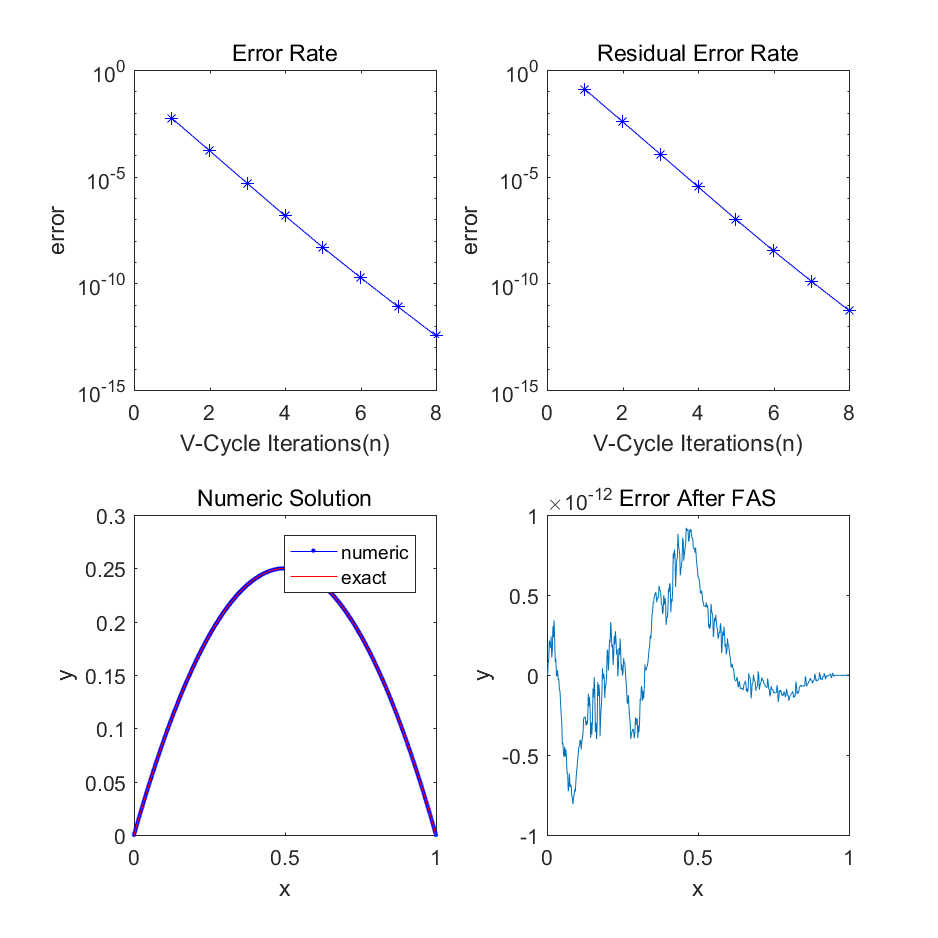
\includegraphics[width=\textwidth]{figure1.png}

\subsection*{问题 II: $f_2(x) = (x^2 + 3x)\me^x + \gamma (x^4 - 2x^2 + x)\me^{2x}$}
此时问题的精确解 $u_2(x) = x(1-x)\me^x$。计算结果与计算时间如下:

\begin{tabular}{r|cccccc}
    \toprule
    $\gamma$        & 0        & 1        & 10       & 25       & 35       & 39       \\
    \midrule
    V-cycle 次数(n) & 8        & 8        & 9        & 12       & 13       & 11       \\
    计算时间(s)     & 0.077732 & 0.078832 & 0.095345 & 0.119505 & 0.118348 & 0.101846 \\
    \bottomrule
\end{tabular}

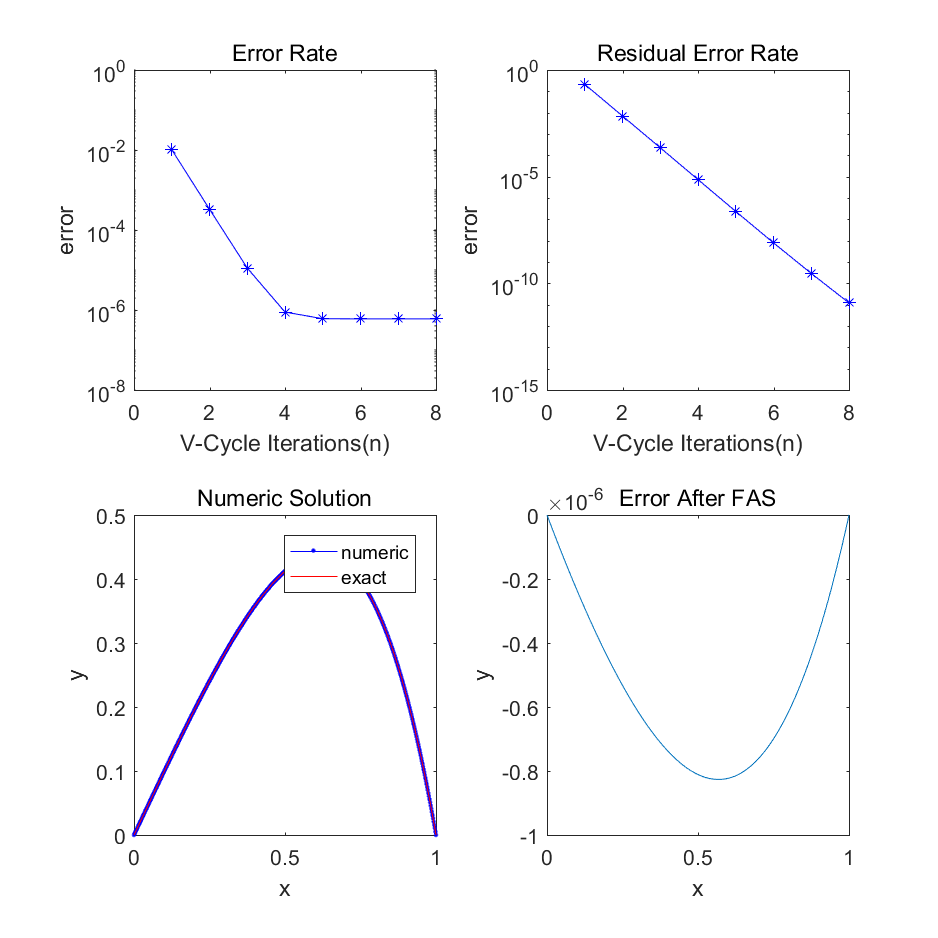
\includegraphics[width=\textwidth]{figure2.png}
%------------------------------------------------------------------------------%


%------------------------------------------------------------------------------%
\subsection*{计算环境}
\begin{tabular}{r|l}
    \hline
    CPU    & \ Intel(R) Core(TM) i7-6700 CPU @ 3.40GHz \\
    \hline
    RAM    & \ 8 GB                                    \\
    \hline
    OS     & Windows 10 Home, x64                      \\
    \hline
    Matlab & Matlab 2016b, Version 9.1.0.441655        \\
    \hline
\end{tabular}
%------------------------------------------------------------------------------%


%------------------------------------------------------------------------------%
\section{多重网格方法}
多重网格方法最早由 R. P. Fedorenko\cite{Fedorenko1962A} 于上世纪60年代提出并逐
渐发展成型。一开始只是用于求解一般的椭圆方程,随后逐渐发展为一个通用的求解偏微
分方程组的方法。从求解的方程类型来看,不仅可以对一般的线性方程进行求解,同样也
可以对非线性的问题进行求解(如算例)。同样,由于最终的问题是求解代数方程,所以
多重网格方法不仅可以与一般的有限差分法结合,也可以与有限元方法结合。简而言之,
首先在细网格上利用迭代法对原代数方程进行第一次求解(松弛),然后在粗网格上利用
迭代法对残差方程进行第二次求解(松弛),从而将残差解反馈给细网格进行校正,这便
是一次简单的多重网格的迭代过程。而通过反复的使用这一迭代过程,从而得到最终的结
果。

多重网格方法的计算形式简单,其核心在于用残差方程的解对原始解进行校正,而核心的
方程求解过程即便是选用简单的迭代法,也能达到较高的收敛速度。而在第五章中,通过
讨论加权平均算子 $I_{h}^{2h}$ 和插值算子 $I_{2h}^{h}$ ,得到了一般的双网格校正
方法在误差与收敛速度上的表现的合理性解释:在一次无松弛的双网格计算之后(对应书
中的算子 $TG$ p82-83),误差中的光滑模(低频模段)表现为光滑模和振荡模,但是增
幅 $s_k = \sin^2 (\frac{\pi k}{2n}) \approx O(\frac{k^2}{n^2}), k \ll n$,
因此双网格矫正法在处理误差中的光滑项表现出色。而在针对振荡模(高频模段)同样会
得到光滑模和振荡模,而增幅
$c_k = \cos^2 (\frac{\pi k}{2n}) \approx O(1-\frac{k^2}{n^2}), k \ll n$,
所以无松弛的双网格校正方法并不能有效地对高频误差进行约简。

而在加入 $\nu$ 次松弛之后,不妨设 $\lambda_k$ 是松弛方法的矩阵 $\mmr$ 对应的的
第 $k$ 个特征值,那么对于误差的第 $k$ 模 $\mvw_k$ 有

\begin{align}
    TG \mvw_k & = \lambda_k^{\nu} s_k \mvw_k + \lambda_k^{\nu} s_k \mvw_{k'} \\
    TG \mvw_k & = \lambda_k^{\nu} c_k \mvw_k + \lambda_k^{\nu} c_k \mvw_{k'} \\
    k'        & = n - k, 1 \le k \le \frac{n}{2} \notag
\end{align}

从而通过所选用的松弛法的收敛能力对双网格校正方法进行辅助,从而改善原有方法在高
频段的收敛能力不足的缺点。同样得,其他的多重网格方法也可以用类似的方式对其收敛
性与收敛阶数进行证明。

虽然多重网格方法在低频上的收敛能力很强,但是实际上很多简单的迭代法同样在低频上
具有较好的收敛能力(第二章的部分例题),所以低频的强收敛能力并非多重网格方法的
优势。同时注意到,实际上左右多重网格的收敛能力的方法是其核心所选择的迭代法自身
的收敛能力。也就是说,选择恰当的迭代法,才是在相同大小的网格上提高其计算精度的
唯一方法。另外值得注意的是,由于多重网格方法的核心在于用残差方程的解对原方程进
行校正,所以其最大的优势在于计算时间的开销很少。具体而言,如
$FMG(\nu_1, \nu_2)$ 方法,选用 Gauss-Seidel 迭代法,其时间复杂度为
$O(k (\nu_1 + \nu_2) V)$,其中 $k$ 表示 FMG 实施的次数,$V$ 表示空间网格数。由
于一般 $\nu_1, \nu_2$ 均取较小的常数值,而一般 $k$ 满足 $k \ll V$,所以实际上
其时间消耗几乎与网格数成线性关系。而一般的迭代法却不能总保证迭代次数 $iter$ 满
足 $iter \ll V$ ,所以往往一般的迭代法的计算速度较慢。

另外值得注意的是,在计算空间的存储上,多重网格方法并不占优势。即便是朴素的迭代
法,通过一些简单的技巧,可以在求解线性方程组时,将其空间复杂度约简至 $O(V)$,
其中 $V$ 表示空间网格数。而注意到,不论是 V-Cycle ,还是 FMG ,其空间复杂度均
为 $O(\beta V)$ ,其中 $\beta = 2(1-2^{-d})^{-1}, (V-Cycle)$,
$\beta = 2(1-2^{-d})^{-2}, (FMG)$ , $d$ 表示解空间的维数。之所以将常数
$\beta$ 单独列出,是因为其与解空间维数相关,而且维数越大其空间复杂度越小。另外
对于维数为 1 的时候,两者分别是 $\varTheta(4 V)$ 和 $\varTheta(8 V)$ ,其空间
开销几乎对应了额外加密 4 倍的朴素迭代法的消耗。但是考虑到其计算速度的优势,这
些额外的空间开销完全可以忍受。

最后一点,多重网格方法可以对非线性的方程进行求解,并且能保证一定的求解精度与收
敛速度。实质上,和前文类似,如果选用非线性的迭代法,如牛顿法,利用多重网格的校
正格式,便可以对非线性方程进行求解,之前的数值算例便是一个很好的例子。

\nocite{Briggs2000A, Oh2005A, Brandt2003Multigrid}
%------------------------------------------------------------------------------%

\phantomsection
\addcontentsline{toc}{section}{参考文献}
\bibliographystyle{nputhesis}
\bibliography{reference}
\end{document}